\documentclass[11pt,a4paper]{article}

% Packages
\usepackage[utf8]{inputenc}
\usepackage[margin=1in]{geometry}
\usepackage{graphicx}
\graphicspath{{Presentation/}{./}}
\usepackage{amsmath,amssymb}
\usepackage{booktabs}
\usepackage{xcolor}
\usepackage{colortbl}
\usepackage{hyperref}
\usepackage{float}
\usepackage{caption}
\usepackage{subcaption}
\usepackage{enumitem}
\usepackage{titlesec}
\usepackage{fancyhdr}
\usepackage{tikz}
\usetikzlibrary{shapes,arrows,positioning}
\usepackage{listings}
\usepackage{makecell}
\usepackage{multirow}
\usepackage{tocloft}
\setcounter{tocdepth}{2}  % Only show sections and subsections in TOC
\renewcommand{\cftsecfont}{\normalsize}
\renewcommand{\cftsubsecfont}{\small}
\renewcommand{\cftsecpagefont}{\normalsize}
\renewcommand{\cftsubsecpagefont}{\small}
\setlength{\cftbeforesecskip}{5pt}
\setlength{\cftbeforesubsecskip}{2pt}

% Illinois Brand Colors
\definecolor{IlliniOrange}{HTML}{FF5F05}
\definecolor{IlliniBlue}{HTML}{13294B}

% Hyperref setup
\hypersetup{
    colorlinks=true,
    linkcolor=IlliniBlue,
    citecolor=IlliniBlue,
    urlcolor=IlliniBlue
}

% Section formatting
\titleformat{\section}
  {\color{IlliniBlue}\Large\bfseries}{\thesection}{1em}{}
\titleformat{\subsection}
  {\color{IlliniBlue}\large\bfseries}{\thesubsection}{1em}{}
\titleformat{\subsubsection}
  {\color{IlliniBlue}\normalsize\bfseries}{\thesubsubsection}{1em}{}

% Header and footer
\pagestyle{fancy}
\fancyhf{}
\fancyhead[L]{\color{IlliniBlue}\small AAD for Second-Order Greeks}
\fancyhead[R]{\color{IlliniBlue}\small Summary Report}
\fancyfoot[C]{\thepage}
\renewcommand{\headrulewidth}{0.5pt}
\renewcommand{\footrulewidth}{0pt}

% Code listing style
\definecolor{codegreen}{rgb}{0,0.6,0}
\definecolor{codegray}{rgb}{0.5,0.5,0.5}
\definecolor{backcolour}{rgb}{0.95,0.95,0.92}
\lstdefinestyle{mystyle}{
  backgroundcolor=\color{backcolour},
  commentstyle=\color{codegreen},
  keywordstyle=\color{blue},
  numberstyle=\tiny\color{codegray},
  basicstyle=\ttfamily\footnotesize,
  breaklines=true,
  keepspaces=true,
  numbers=left,
  numbersep=5pt,
  showstringspaces=false,
  tabsize=2
}
\lstset{style=mystyle}

% Title
\title{
  \color{IlliniBlue}\textbf{Second Order Greeks via\\Adjoint Algorithmic Differentiation}\\
  \vspace{0.5em}
  \large Summary Report
}
\author{
  Junru Wang \quad Zhaolin Shi \quad Zhengtao Yu\\
  Yaru Guan \quad Zilin Mao \quad Wenqi Guo\\[0.5em]
  \small Master of Science in Financial Engineering\\
  \small University of Illinois at Urbana-Champaign\\
  \small \textit{Corporate Advisor: Gan Wang, Vicky Luo (JPMorgan Chase)}\\
  \small \textit{Instructor: Prof. Feng}
}
\date{December 12, 2025}

\begin{document}

\maketitle
\thispagestyle{empty}

\newpage
\thispagestyle{empty}

\begin{center}
{\Large\bfseries\color{IlliniBlue} Abstract}
\end{center}
\vspace{1em}

\noindent
This report presents a comprehensive implementation of Adjoint Algorithmic Differentiation (AAD) for computing second-order Greeks in financial derivatives pricing. We developed a tape-based reverse-mode automatic differentiation framework with three Hessian computation methods: \textbf{Edge-Pushing} for sparse Hessians, \textbf{Taylor Expansion} for dense Hessians, and \textbf{Bumping2} (finite difference) for validation. Our implementation achieves up to \textbf{42$\times$ speedup} over traditional finite difference methods for PDE-based pricing with B-spline local volatility surfaces. The framework has been validated on real SPX options data with 5,405 contracts.

\vspace{2em}

\noindent\textbf{Key Words:} Adjoint Algorithmic Differentiation (AAD), Second-Order Greeks, Hessian Computation, Edge-Pushing Algorithm, Taylor Expansion, B-spline Local Volatility, Monte Carlo Simulation, PDE Pricing, Cython Optimization, Financial Derivatives

\newpage
\thispagestyle{empty}

\begin{center}
{\Large\bfseries\color{IlliniBlue} Executive Summary}
\end{center}
\vspace{1em}

\noindent
This practicum project, sponsored by JPMorgan Chase, developed a production-ready Adjoint Algorithmic Differentiation (AAD) framework for computing second-order Greeks (Gamma, Vanna, Volga) in financial derivatives pricing. Traditional finite-difference ``bumping'' methods scale poorly with parameter dimensionality, requiring $O(n^2)$ re-pricings to compute a full Hessian matrix. Our AAD-based approach reduces this to $O(1)$ pricing evaluations, achieving dramatic computational savings.

\vspace{1em}
\noindent\textbf{Key Technical Achievements:}
\begin{itemize}[leftmargin=*]
  \item \textbf{Core AAD Engine:} Implemented a tape-based reverse-mode automatic differentiation system with Python operator overloading, enabling seamless integration with existing pricing models.
  \item \textbf{Edge-Pushing Algorithm:} Developed an efficient sparse Hessian computation method that exploits the locality of B-spline basis functions, achieving \textbf{42$\times$ speedup} over finite differences for PDE-based calibration.
  \item \textbf{Taylor Expansion Method:} Implemented an alternative dense Hessian approach particularly suited for Monte Carlo simulations with correlated paths.
  \item \textbf{Cython Optimization:} Achieved \textbf{12$\times$ performance improvement} over pure Python through compiled Cython extensions.
  \item \textbf{Real Data Validation:} Successfully calibrated B-spline local volatility surfaces on SPX options (5,405 contracts, $S_0 = \$6081.76$) with Hessian errors in the range $10^{-8}$ to $10^{-14}$.
\end{itemize}

\vspace{1em}
\noindent\textbf{Business Impact:}
\begin{itemize}[leftmargin=*]
  \item \textbf{Risk Management:} Enables real-time computation of second-order sensitivities for large portfolios, supporting more accurate hedging strategies.
  \item \textbf{Model Calibration:} Provides exact Hessians for second-order optimization methods (Newton, L-BFGS), improving convergence speed and robustness.
  \item \textbf{Scalability:} Framework handles high-dimensional parameter spaces (tested up to 40 assets) where finite differences become computationally prohibitive.
\end{itemize}

\vspace{1em}
\noindent\textbf{Recommendations:}
The Edge-Pushing method is recommended for PDE-based pricing with structured parameter spaces (B-splines, piecewise models), while Taylor Expansion is preferred for Monte Carlo simulations with dense Hessians. Future enhancements include GPU acceleration for large-scale simulations and checkpointing for memory-constrained environments.

\newpage
\tableofcontents
\newpage
\section{Introduction}
%=============================================================================

Modern risk management for large derivative portfolios requires accurate and timely
computation of sensitivities with respect to a high-dimensional set of model parameters.
In practice, these sensitivities, commonly referred to as Greeks, are used for hedging,
capital allocation, stress testing, and model calibration. As financial models grow in complexity, incorporating Monte Carlo simulation, partial
differential equation (PDE) solvers, and high-dimensional volatility parameterizations,
the computational burden of traditional sensitivity analysis has become a critical
bottleneck in production risk systems, often rendering higher-order Greeks prohibitively
expensive or altogether unavailable in time-sensitive risk and hedging workflows.


\subsection{Project Motivation}

From the perspective of a large investment bank such as J.P. Morgan, the dominant industry
approach for computing Greeks remains finite-difference bumping. While conceptually simple,
bumping scales poorly: computing $n$ first-order Greeks requires $O(n)$ full re-valuations,
and computing a full Hessian of second-order Greeks requires $O(n^2)$ re-pricings. For
models that already involve expensive numerical engines, such as Monte Carlo simulations
with early exercise features or PDE solvers with local volatility surfaces, this quadratic
scaling quickly becomes infeasible in real-time or overnight risk pipelines.

Adjoint Algorithmic Differentiation (AAD) has emerged over the past decade as a promising
alternative. Reverse-mode AAD exploits the structure of the computation graph underlying a
pricing function to compute all first-order sensitivities in a single backward sweep,
with computational cost largely independent of the number of input parameters. Extending
this efficiency to second-order Greeks, however, is substantially more challenging. Na\"ive
extensions of reverse-mode AAD either suffer from prohibitive memory usage or lose the
computational advantages that make AAD attractive in the first place.

This challenge is of direct interest to the project sponsor. Second-order Greeks such as
Gamma, Vanna, and Volga play a central role in nonlinear risk management, model calibration,
and hedging under stressed market conditions. In many production environments, however,
these quantities are computed only approximately or are excluded altogether, as their
evaluation requires a prohibitively large number of re-valuations when using conventional
finite-difference methods. Developing a practical and scalable framework for computing
second-order Greeks, while remaining compatible with realistic pricing engines and real
market data, therefore addresses a concrete and high-impact problem faced by front-office
quantitative risk teams.


\subsection{Project Scope}
The scope of this project is to design, implement, and validate a unified AAD-based
framework for the efficient computation of both first-order and second-order Greeks in
modern derivatives pricing models. We adopt reverse-mode AAD as the core differentiation
paradigm and investigate two complementary techniques for Hessian computation, namely
the Edge-Pushing algorithm for sparse Hessians and the Taylor Expansion method for dense
Hessians. These methods are integrated into both PDE-based and Monte Carlo-based pricing
engines and are evaluated against traditional finite-difference benchmarks.


\subsection{Team Objectives}

To achieve the goals outlined above, the project is organized around the following
objectives:
\begin{itemize}
  \item Develop a tape-based reverse-mode AAD engine using Python operator overloading,
        enabling systematic construction and traversal of computation graphs.
  \item Implement the Edge-Pushing algorithm to compute second-order derivatives efficiently
        by exploiting sparsity in structured models such as B-spline local volatility PDEs.
  \item Implement a Taylor Expansion–based differentiation engine to handle dense Hessians
        arising in Monte Carlo simulations.
  \item Integrate the AAD framework with multiple pricing engines, including
        Crank--Nicolson PDE solvers and Monte Carlo basket option pricers.
  \item Address non-smooth payoffs and early exercise features using smoothing techniques
        and frozen exercise-time strategies suitable for higher-order differentiation.
  \item Optimize the implementation for practical performance using Cython acceleration
        and memory-aware design choices.
  \item Validate accuracy and scalability against finite-difference benchmarks and apply
        the framework to real SPX options data.
\end{itemize}

\subsection{Summary of Key Contributions}

The project delivers a production-oriented AAD framework capable of computing second-order
Greeks with substantial performance gains over finite-difference methods. For PDE-based
calibration with B-spline local volatility surfaces, the Edge-Pushing algorithm achieves up
to a $42\times$ speedup by exploiting Hessian sparsity, requiring only a single PDE solve
regardless of parameter dimension. For Monte Carlo pricing, the Taylor Expansion method
provides an efficient and stable approach to dense Hessian computation. Through Cython
optimization, the core AAD engine attains an additional $12\times$ speedup over pure Python
implementations. The framework is validated on real SPX options data comprising 5,405
contracts, demonstrating both numerical accuracy and practical scalability.


\subsection{Organization of the Report}

The remainder of this report is organized as follows.
First, Section~2 introduces the theoretical foundations of automatic differentiation,
reverse-mode AAD, and the algorithms used for second-order derivative computation,
including Edge-Pushing and Taylor Expansion.
Second, Section~3 describes the system architecture and implementation details of the
AAD framework, with particular emphasis on optimization strategies and integration with
both PDE-based and Monte Carlo-based pricing engines.
Third, Section~4 presents numerical results, including accuracy and runtime benchmarks
under PDE and Monte Carlo settings, as well as validation using real market data.
Finally, Section~5 concludes with a comparative summary of methods, key findings, and
directions for future work.
%=============================================================================
\section{Methodology}
%=============================================================================

% 于郑韬 Dec 5 修改从此开始
\subsection{Automatic Differentiation: Concepts}

Automatic Differentiation (AD) is a computational technique for evaluating derivatives
of functions that are implemented as computer programs.  
The term “automatic’’ highlights the fact that, once the computational structure of a
function has been specified, its derivatives can be obtained systematically and with
machine precision, without resorting to symbolic manipulation or numerical finite
differences.

\paragraph{Insight of “Automatic”}

At the core of AD lies a simple but powerful observation: any computer program
can be decomposed into a sequence of \emph{elementary operations}, such as
addition, multiplication, exponential, logarithm, and so on.  
For each such elementary operation, the corresponding mathematical derivative
is known analytically.  
This means that, once a program is expressed as a composition of these atomic
operations, AD can apply the chain rule in a structured and mechanical way
throughout the computation.

In contrast to symbolic differentiation, AD does not manipulate algebraic expressions; 
instead, it operates directly on numerical values and intermediate variables generated
during program execution.  
And unlike finite-difference methods, AD introduces no truncation error beyond
machine precision.  As a result, AD provides a highly reliable and efficient method 
for computing sensitivities.

\paragraph{Modes of Automatic Differentiation}

There are two principal modes of AD, each suited to different computational settings.

\subparagraph{Forward Mode}

Forward mode AD propagates derivatives \emph{alongside} the primal values.
During the evaluation of a program, every intermediate variable carries not only its
numerical value but also its derivative with respect to a chosen input direction.
This approach is efficient when the number of input variables $n$ is small, because
each execution of the program yields one directional derivative.  
Thus, computing a full gradient requires $n$ forward passes.

\subparagraph{Reverse Mode}

Reverse mode AD, also known as adjoint algorithmic differentiation (AAD), proceeds
in the opposite direction.  
The program is evaluated once in a forward pass, during which intermediate values
and local Jacobians are recorded.  
A subsequent backward sweep propagates \emph{adjoint} variables from the output
back toward the inputs.  
Crucially, a single reverse pass produces the entire gradient, regardless of the number
of input variables.

This asymmetry makes reverse mode particularly advantageous in applications where
\[
\text{number of inputs} \gg \text{number of outputs},
\]
which is the case in many financial models where a scalar objective—such as a price,
risk metric, or loss function—depends on a high-dimensional set of underlying
parameters.  
In such settings, reverse mode AD can compute all first-order sensitivities orders of
magnitude faster than finite-difference bumping.


\paragraph{Illustrative Example}

To visualize how AD operates over a program, it is helpful to examine its computation
graph.  
Figure~\ref{fig:lognormal_graph} shows the expression graph for the log-normal
density function,
\[
f(y;\mu,\sigma)
= \frac{1}{y \sigma \sqrt{2\pi}}
  \exp\!\left(
    -\frac{(\ln y - \mu)^2}{2\sigma^2}
  \right).
\]
Each node in the graph represents an elementary operation, and edges indicate
data dependencies and the flow of intermediate values.  
Such computational graphs are typically directed acyclic graphs (DAGs), ensuring
that derivatives can be propagated unambiguously in either forward or reverse mode.


\begin{figure}[ht]
    \centering
    \includegraphics[width=0.55\textwidth]{lognormal_density_graph.png}
    \caption{Computation graph for the log-normal density function. 
    (The indexing of nodes follows the Wengert list notation introduced later.)}
    \label{fig:lognormal_graph}
\end{figure}

This decomposition into elementary operations is exactly what enables AD to apply
the chain rule automatically, leading to efficient and accurate computation of
gradients and, as shown later, higher-order derivatives such as Hessians.

\subsection{Computation Graph}

Automatic Differentiation relies on an explicit representation of how a numerical
program is composed from elementary operations.  
This representation is known as a \emph{computation graph}, which encodes both the
data dependencies among intermediate variables and the structure required for
applying the chain rule in forward or reverse mode.

\paragraph{Wengert List Notation}

To express the computation graph in a form that facilitates differentiation,
we adopt the classical \emph{Wengert list} (also known as a Wengert tape).
In this notation, the independent variables are indexed as
\[
v_{-n}, \dots, v_{-1}, v_0,
\]
while each elementary operation in the program produces a new state variable
\[
v_1, v_2, \dots, v_\ell.
\]
Together, these registers form the \emph{state vector} of the computation.

This indexing convention provides a unified way to represent inputs,
intermediate quantities, and the final output within a single ordered sequence.
It is particularly convenient for reverse-mode differentiation and for the
second-order constructions introduced later, where the Hessian expressions
naturally reference variables using this Wengert indexing scheme.

\paragraph{Edges}

An edge in a computation graph represents a function argument—that is, a dependency
between two operations.  
Edges simply indicate where each node receives its inputs; they do not contain
numerical information by themselves.  
In this sense, edges serve as pointers that organize the direction of data flow
through the program.

\paragraph{Nodes}

Nodes correspond to elementary operations such as addition, multiplication,
logarithm, or exponentiation.  
The head node of an edge is a function of its tail node, which encodes the composition
structure of the program.

Each node also “knows’’ its own local derivatives.  
This means that, for every operation, AD stores both the value of the operation and
its partial derivatives with respect to its inputs.  
During reverse-mode differentiation, the node multiplies the incoming adjoint by its
local Jacobian, implementing the chain rule
\[
\frac{\partial F}{\partial u}
    =
    \frac{\partial F}{\partial v}
    \cdot
    \frac{\partial v}{\partial u}.
\]
This local derivative information is what enables AD to propagate gradients efficiently
through the entire graph.

\paragraph{Tape Representation}

While edges and nodes define the static structure of the computation graph, AD
systems also maintain a \emph{tape}—a runtime record generated during the forward pass.  
After one evaluation of the program, the tape contains:
\begin{enumerate}
    \item the topological order of nodes (i.e., the predecessor structure),
    \item all forward values computed along the way, and
    \item the numerical Jacobians or gradients associated with each elementary operation.
\end{enumerate}
This information is exactly what the reverse sweep requires to apply the chain rule
backward from the output to the inputs.

\paragraph{Illustrative Example}

Figure~\ref{fig:lognormal_graph} presents the computation graph for the log-normal
density function,
\[
f(y;\mu,\sigma)
= 
\frac{1}{y\sigma\sqrt{2\pi}}
\exp\!\left(
   -\frac{(\ln y - \mu)^2}{2\sigma^2}
\right).
\]
The graph shows how the function decomposes into a sequence of elementary operations,
each represented by a single node.  
Edges express the dependencies between intermediate results, and the entire graph
forms a \emph{directed acyclic graph (DAG)}, ensuring that computations proceed in
a well-defined order.



Understanding this graph representation is essential for both first-order AD and the
higher-order techniques, such as the edge-pushing algorithm, discussed later in this
report.

\subsection{Reverse-Mode AAD: Efficiency and Extensions to Hessians}

Reverse-mode Automatic Differentiation (AD), also referred to as Adjoint Algorithmic
Differentiation (AAD), plays a central role in the computation of sensitivities in financial
models.  In this section, we review its efficiency for first-order Greeks and explain how
its principles can be extended to second-order derivatives.

\paragraph{First-Order Greeks}

In practice, the simplest and most widely used method for computing sensitivities is
finite-difference bumping.  
For each input parameter $x_i$, a perturbed evaluation is required:
\[
   \Gamma_i \;\approx\; \frac{F(x + h e_i) - F(x)}{h},
\]
where $h$ is a small bump size and $e_i$ is the $i$-th unit vector.  
This approach must be repeated for every parameter, making it computationally costly
when the dimension of the input vector is large.

By contrast, reverse-mode AAD evaluates the entire gradient in a \emph{single} backward
sweep.  
After one forward pass that records the necessary intermediate values and local
Jacobians, the adjoint variables propagate from the output back toward the inputs.  
This single reverse pass yields all first-order Greeks simultaneously.

\paragraph{Time Complexity Considerations}

The computational advantage of reverse-mode AAD becomes clear when comparing
complexity.  
Finite-difference bumping requires $\mathcal{O}(n)$ evaluations of the pricing
function, where $n$ is the number of input parameters.  
Reverse-mode AAD, however, requires:
\begin{itemize}
    \item one forward evaluation of the pricing function, and
    \item one backward sweep whose cost does not scale with $n$.
\end{itemize}
Thus the overall complexity of AAD is effectively $\mathcal{O}(1)$ with respect to the
input dimension, making it dramatically more efficient when
\[
\text{number of inputs} \gg \text{number of outputs}.
\]
This asymmetry is typical in risk and pricing applications where models depend on a
large set of risk factors but return a single scalar output.

\paragraph{Beyond First Order: Towards Hessians}

While reverse-mode AAD provides an efficient mechanism for computing gradients,
extending these ideas to second-order derivatives (Hessians or second-order Greeks)
is not straightforward.  
To address this challenge, we follow the framework introduced by Gower and Mello
(2012), who developed a systematic method for propagating second-order information
through a computation graph.

A key component of their framework is the \textbf{edge-pushing algorithm}, which
implements a second-order chain rule and transports curvature information along the
graph during a node-sweeping process.  
This algorithm allows Hessian blocks to be constructed efficiently by combining
Jacobian products and local second derivatives at each node.

Throughout this project, finite-difference bumping serves as the benchmark method
against which we compare the performance and accuracy of the edge-pushing
approach.  Although bumping is simple and widely used, its computational cost grows
quadratically for Hessians, making it an ideal reference point for evaluating the
efficiency gains provided by second-order AD techniques.

\subsection{Hessian Computation via State Transformations and Edge-Pushing}

In order to derive an efficient procedure for computing second-order derivatives, we
begin by expressing the target function in a structured form that reflects its computation
graph.  This formulation follows the framework of Gower and Mello (2012), which
provides a convenient algebraic representation for the application of second-order
automatic differentiation.

\paragraph{Function Representation and State Transformations}

Let $x \in \mathbb{R}^n$ denote the input vector.  
We embed $x$ into an extended state space through the matrix
\[
P = [I_n \;\; 0], \qquad P^\top x = (x,0,\ldots,0) \in \mathbb{R}^{n+\ell}.
\]
The computation of the function proceeds by applying a sequence of state
transformations,
\[
f(x) = e_\ell^\top (\Phi_\ell \circ \cdots \circ \Phi_1)(P^\top x),
\]
where each transformation $\Phi_i$ updates only a single component of the state
vector.  
This reflects the fact that an elementary operation in a computation graph affects
only one intermediate variable at a time.

The vector $e_\ell^\top$ simply extracts the final register, representing the scalar output
of the computation.

\paragraph{Second-Order Chain Rule}

The Hessian of $f$ can be written compactly as
\[
f''(x)
=
P \Bigg(
\sum_{i=1}^{\ell}
  \Big( \prod_{j=1}^{i-1} (\Phi_j')^\top \Big)
  \big( (\bar{v}^i)^\top \Phi_i'' \big)
  \Big( \prod_{j=1}^{i-1} \Phi_{i-j}' \Big)
\Bigg)
P^\top,
\]
where:

\begin{itemize}
    \item $\Phi_i'$ and $\Phi_i''$ denote the local Jacobian and Hessian at node $i$,
    \item $\bar{v}^i$ is the adjoint variable obtained during reverse-mode propagation,
    \item $P$ and $P^\top$ map between input space and the extended state space.
\end{itemize}

This expression shows that each nonlinear operation contributes a term that is
sandwiched between products of Jacobians, reflecting the transport of curvature
through the computation graph.

\paragraph{Block Form}

To simplify notation, define
\[
f''(x) = P W P^\top, \qquad W = \sum_{i=1}^{\ell} W_i.
\]
Each summand $W_i$ corresponds to the curvature generated at node $i$ and transported
through the graph via Jacobian factors.

The $(i-1)$-th summand has the form
\[
W_{i-1} =
\Big((\Phi_1')^\top \cdots (\Phi_{i-2}')^\top \Big)
  (\bar{v}^{\,i-1})^\top
  \Phi_{i-1}''
\Big( \Phi_{i-2}' \cdots \Phi_1' \Big),
\]
while the $i$-th summand is similar but includes additional Jacobian factors,
\[
W_i =
\Big((\Phi_1')^\top \cdots (\Phi_{i-2}')^\top \Big)
  (\Phi_{i-1}')^\top
  (\bar{v}^{\,i})^\top
  \Phi_{i}''
  \Phi_{i-1}'
\Big( \Phi_{i-2}' \cdots \Phi_1' \Big).
\]
The structural similarity between consecutive $W_i$ terms motivates an iterative
construction.

\paragraph{Three-Step Logic for Iterative Construction}

Because each $W_i$ can be built from $W_{i-1}$ using only local Jacobian and Hessian
information, the Hessian construction decomposes naturally into three steps:
\begin{enumerate}
    \item \textbf{Push Step:}
    Propagate existing second-order information via
    \[
    W \gets (\Phi_i')^\top W \Phi_i'.
    \]
    \item \textbf{Create Step:}
    Add new second-order contributions generated at node $i$,
    \[
    W \gets W + \bar{v}^\top \Phi_i''.
    \]
    \item \textbf{Update Step:}
    Update the adjoint variable using the local Jacobian,
    \[
    \bar{v}^\top \gets \bar{v}^\top \Phi_i'.
    \]
\end{enumerate}

These three operations—Push, Create, and Update—form the core of the
\emph{edge-pushing algorithm}, which computes Hessians in a single sweep through
the computation graph.

\paragraph{Componentwise Interpretation on a Computation Graph}

The edge-pushing procedure becomes particularly intuitive when viewed directly on a
computation graph.  
As nodes are swept in reverse topological order, nonlinear arcs representing
second-order dependencies are created, pushed, and updated.

For example, consider the function
\[
f(x) = (x_{-2} + e^{x_{-1}})(3x_{-1} + x_0^2).
\]
Sweeping node 3 creates a nonlinear arc $\{1,2\}$.  
Sweeping node 2 pushes and splits this arc into $\{0,1\}$ with weight $1\cdot 2v_0$
and $\{-1,1\}$ with weight $1\cdot 3$.  
Sweeping node 1 pushes the latter arc into $\{-2,-1\}$ and $\{-1,-1\}$, the latter
accumulating weight $2\cdot 3 \cdot e^{v_{-1}}$.  
Local curvature $\partial^2 \phi_1 / \partial v_{-1}^2$ is added to the arc $\{-1,-1\}$
during the same sweep.

Figure~\ref{fig:ep_graph} illustrates these operations graphically.

\begin{figure}[ht]
    \centering
    \includegraphics[width=1\textwidth]{ep_illustration}
    \caption{Edge-pushing applied to a computation graph.}
    \label{fig:ep_graph}
\end{figure}

At the end of the sweep, the Hessian entries are obtained from the weights assigned
to nonlinear arcs between independent nodes.



\subsection{Taylor Expansion for Dense Hessians}

Taylor Expansion provides an alternative second-order differentiation technique in which
each node of the computational graph carries a local truncated Taylor series. Instead of
propagating second-order edge pairs as in Edge-Pushing, Taylor Expansion generates all
required monomials through a single forward sweep. This makes it particularly suitable for
dense Hessians arising in Monte Carlo simulations.

Each AD variable stores a triple $(v_0, v_1, v_2)$:
\begin{itemize}
  \item $v_0$: Function value
  \item $v_1$: First-order Taylor coefficient (gradient contribution)
  \item $v_2$: Second-order Taylor coefficient (quadratic contribution)
\end{itemize}

Formally, for an infinitesimal perturbation $\varepsilon$ applied to the output,
\[
v(\varepsilon) = v_0 + \varepsilon v_1 + \tfrac{1}{2}\varepsilon^2 v_2 + O(\varepsilon^3),
\]
so $(v_0,v_1,v_2)$ represents the truncated Taylor expansion of each intermediate variable
with respect to a single seed.

\paragraph{Forward Taylor Propagation.}
For every elementary operation $y = \phi(x_1,\dots,x_m)$, we apply the second-order Taylor
rule
\[
y(\varepsilon)
= \phi(x(\varepsilon))
= \phi(x_0)
+ \varepsilon\,\phi'(x_0) x_1
+ \tfrac{1}{2}\varepsilon^2\left(
  \phi''(x_0)x_1^2 + \phi'(x_0)x_2
\right)
+ O(\varepsilon^3),
\]
which yields the update
\[
y_0 = \phi(x_0), \qquad
y_1 = \phi'(x_0)x_1, \qquad
y_2 = \phi'(x_0)x_2 + \phi''(x_0)x_1^2.
\]
These rules are operator-local and require no knowledge of the global graph structure.

\paragraph{Backward Series Substitution.}
After the forward sweep generates Taylor triples for all nodes, we seed the output with the
perturbation $R + \varepsilon_R$ and express $\varepsilon_R$ in terms of perturbations of
intermediate variables. For example, for
\[
R = \exp(Q), \qquad Q = \cos(P),
\]
the truncated Taylor expansions give:
\[
\varepsilon_R
  = \exp'(Q)\,\varepsilon_Q
  + \tfrac{1}{2}\exp''(Q)\,\varepsilon_Q^2,
\]
\[
\varepsilon_Q
  = \cos'(P)\,\varepsilon_P
  + \tfrac{1}{2}\cos''(P)\,\varepsilon_P^2.
\]
By repeatedly substituting these series (Arbogast’s ``substitution of a series in a series’’),
we express $\varepsilon_R$ as a polynomial in the leaf perturbations
$\varepsilon_{V_i}$.  

For example, if $P = V_1 V_2$, then
\[
\varepsilon_P
= V_2 \varepsilon_{V_1}
+ V_1 \varepsilon_{V_2}
+ \varepsilon_{V_1} \varepsilon_{V_2},
\]
from which all mixed monomials $\varepsilon_{V_i}\varepsilon_{V_j}$ are generated automatically.

Matching the coefficients of $\varepsilon_{V_i}$ and $\varepsilon_{V_i}\varepsilon_{V_j}$
yields the gradient and Hessian.  
Symmetry of the Hessian follows automatically because all second-order monomials are
generated locally during substitution.

\begin{table}[H]
\centering
\caption{Edge-Pushing vs Taylor Expansion Comparison}
\begin{tabular}{lcc}
\toprule
\textbf{Aspect} & \textbf{Edge-Pushing (EP)} & \textbf{Taylor Expansion} \\
\midrule
Derivative storage & second-order edge pairs
  & local $(v_0,v_1,v_2)$ per node \\
Reverse sweep cost & requires large nonlinear graph
  & \textbf{single backward sweep} \\
Scaling with steps & graph size grows with time
  & \textbf{linear in computational depth} \\
Hessian symmetry & requires explicit enforcement
  & \textbf{automatic by construction} \\
Best use case & sparse PDE Hessians
  & \textbf{dense MC Hessians} \\
\bottomrule
\end{tabular}
\end{table}

\paragraph{Key Advantages.}
Taylor Expansion offers several structural benefits:
\begin{itemize}
  \item \textbf{Locality:} All second-order effects are derived from local operator rules, simplifying implementation.
  \item \textbf{Scalability:} Cost grows linearly with the length of the computational graph, independent of the number of inputs.
  \item \textbf{Dense Hessian efficiency:} No sparsity assumptions are required; dense blocks arise naturally.
  \item \textbf{Symmetry preservation:} Hessian symmetry is inherent, eliminating the need for post-processing.
  \item \textbf{Unified forward--backward workflow:} A single lightweight backward sweep recovers the full Hessian.
\end{itemize}

\textit{Takeaway: Taylor avoids graph blow-up, preserves symmetry, and provides highly scalable
second-order derivatives, making it ideal for dense Monte Carlo Hessians.}


\subsection{B-spline Local Volatility Surface}

We represent the local volatility surface using a tensor–product B-spline basis.  
Let $B_i^{p}(K)$ and $B_j^{q}(T)$ denote univariate B-spline basis functions of
degree $p$ in strike and degree $q$ in maturity.  
The surface takes the form
\begin{equation}
\sigma_{\text{loc}}(K, T; \mathbf{w})
=
\sum_{i=1}^{n_K} \sum_{j=1}^{n_T}
w_{ij} \, B_i^{p}(K)\, B_j^{q}(T),
\end{equation}
where the coefficients $w_{ij}$ control the contribution of each tensor-product
basis function.  
This parametrization produces a smooth and flexible volatility surface while
maintaining local support and differentiability, properties that are essential
for stable calibration and efficient derivative computation.


\subsection{Discontinuous Payoffs}

In real market, options have kink payoff problems. At the strike, classical derivatives do not exist and a naive pathwise AAD through the payoff node returns zero almost surely or yields very
noisy Greeks. In our work, we handle such cases by (i): conditional expectation, vibrato, likelihood ratio, and malliavin integration by parts
——which shift derivatives to the smooth transition density and (ii): kernel or softplus smoothing——which replace the payoff by a smooth surrogate. 


\subsubsection*{Conditional Expectation}

Fix a basket option and a chosen asset direction $k$. Let $S^{(k)}_{N-1}$ be the value of the $k$-th asset at the last step before maturity. We define the last–step conditional expectation:
\begin{equation}
  \varphi_k(x)
  := \mathbb{E}\big[f(S_T)\,\big|\,S^{(k)}_{N-1}=x\big]
  = \int_{\mathbb{R}^d} f(z)\,p_T(z\mid x)\,dz,
\end{equation}
where $p_T(z\mid x)$ is the conditional joint density of $S_T=z$ given
$S^{(k)}_{N-1}=x$. Even if $f$ is nonsmooth in the basket direction, the
transition density $p_T(\cdot\mid x)$ is $C^\infty$ in $x$, so
$\varphi_k(x)$ is smooth and can be differentiated. Conditional expectation thus removes the kink in the chosen direction.

\subsubsection*{Vibrato}
Vibrato uses the score identity:
\begin{equation}
  \nabla_x \varphi_k(x)
  = \mathbb{E}\big[f(X_T)\,\nabla_x \log p_T(X_T\mid x)
    \,\big|\,X_{N-1}=x\big]
\end{equation}
and improves variance by subtracting the baseline $\varphi_k(x)$:
\begin{equation}
  \nabla_x \varphi_k(x)
  = \mathbb{E}\Big[\big(f(X_T)-\varphi_k(x)\big)\,
      \nabla_x \log p_T(X_T\mid x)\,
      \Big|\,X_{N-1}=x\Big],
\end{equation}
since $\mathbb{E}[\nabla_x \log p_T(X_T\mid x)\mid X_{N-1}=x]=0$. Vibrato differentiates the smoothed payoff via the score term, yielding
low–variance first and second derivatives in that direction.

\subsubsection*{Likelihood Ratio Method}

Let $F(x_0)=\mathbb{E}[f(X_T)]$ with $X_0=x_0$ and transition density
$p_T(z;x_0)$. The likelihood ratio method (LRM) moves the derivative inside
the pricing integral:
\begin{equation}
  \frac{dF}{dx_0}
  = \int f(z)\,\partial_{x_0} p_T(z;x_0)\,dz
  = \mathbb{E}\big[f(X_T)\,\partial_{x_0}\log p_T(X_T;x_0)\big].
\end{equation}
This gives the unbiased estimator:
\begin{equation}
  \Delta
  = \mathbb{E}\big[f(X_T)\,w(X_T;x_0)\,\big|\,X_0=x_0\big],
  \qquad
  w(X_T;x_0)=\partial_{x_0}\log p_T(X_T;x_0),
\end{equation}
where the derivative acts on the smooth density $p_T$, not on the nonsmooth
$f$.

\subsubsection*{Malliavin Integration by Parts}
Malliavin integration by parts provides a continuous–time formulation. If
$F=f(X_T)\in\mathbb{D}^{1,2}$ and $U\in L^2([0,T])$, then:
\begin{equation}
  \mathbb{E}\big[\langle DF,U\rangle_{L^2}\big]
  = \mathbb{E}\big[F\,\delta(U)\big],
\end{equation}
with $D_sF=f'(X_T)D_sX_T$ and $\delta(U)$ the Skorokhod integral. Choosing
$U$ so that:
\[
  \langle DX_T,U\rangle_{L^2}=\partial_{x_0}X_T =: G
\]
yields:
\[
  \Delta = \partial_{x_0}\mathbb{E}[f(X_T)] = [f'(X_T)G],
  \qquad
  H_{x_0} = \delta(U).
\]
The integration–by–parts step transfers derivatives from the nonsmooth $f'$ to
the smooth noise via $\delta(U)$, and the final Monte Carlo estimator can be
expressed in terms of $f(X_T)$ only, remaining stable across the strike kink.

\subsubsection*{Kernel Smoothing}

Kernel smoothing regularizes the payoff before applying AAD and Edge-Pushing. Let $\rho$ be a smooth probability density and $\rho_\varepsilon(u)=\varepsilon^{-1}\rho(u/\varepsilon)$ the associated
mollifier, and define:
\[
  f_\varepsilon(x) = (f * \rho_\varepsilon)(x)
  = \mathbb{E}[f(x+\varepsilon Z)], \qquad Z\sim\rho \text{ independent}.
\]
The smoothed price:
\[
  F_\varepsilon(x_0)
  = \mathbb{E}\big[f_\varepsilon(X_T)\big]
  = \mathbb{E}\big[f(X_T+\varepsilon Z)\big]
\]
is differentiable in $x_0$, so:
\[
  \Delta_\varepsilon = \partial_{x_0}F_\varepsilon(x_0), 
  \qquad
  H_\varepsilon = \partial_{x_0}^2F_\varepsilon(x_0)
\]
can be computed by standard reverse–mode AAD on the smooth functional
$F_\varepsilon$. For small $\varepsilon$, $H_\varepsilon$ provides a stable
approximation to the distributional second-order Greeks of the original
discontinuous payoff.






%=============================================================================
\section{Implementation}
%=============================================================================

\subsection{Optimization Stages}

Our implementation evolved through multiple optimization stages to achieve production-ready performance. Table~\ref{tab:optimization_stages} summarizes the technologies used and their relative speedups. We began with a pure Python baseline (Stage 0), which was prohibitively slow for practical use. Stage 1 employed Cython—a hybrid Python/C extension that compiles Python-like code to C—combined with Python's native dictionary for hash-based lookups. This combination achieved a remarkable \textbf{12$\times$ speedup} over the baseline while maintaining development simplicity. We also explored a Stage 2 implementation using C++ \texttt{unordered\_map}, but this yielded only 3.2$\times$ speedup with significantly higher implementation complexity. Based on these results, we deployed Stage 1 (Cython + Python dict) as our production system, demonstrating that careful selection of hybrid technologies can outperform pure low-level implementations.

\begin{table}[H]
\centering
\caption{Implementation Technologies and Performance}
\label{tab:optimization_stages}
\begin{tabular}{@{}llcl@{}}
\toprule
\textbf{Stage} & \textbf{Implementation} & \textbf{Speedup} & \textbf{Status} \\
\midrule
\textbf{Stage 0} & Pure Python & 1.0$\times$ (baseline) & \textcolor{red}{Too slow} \\
\textbf{Stage 1} & Cython + Python dict & \textcolor{green}{\textbf{12.0$\times$}} & \textcolor{green}{$\checkmark$ Deployed} \\
\textbf{Stage 2} & C++ unordered\_map & 3.2$\times$ & \textcolor{orange}{Alternative} \\
\bottomrule
\end{tabular}
\end{table}

\textbf{Key Technologies:}
\begin{itemize}
  \item \textbf{Cython:} Hybrid Python/C extension that compiles Python-like code to C, providing near-C performance while maintaining Python's ease of use.
  \item \textbf{Python dict:} Native Python dictionary with $O(1)$ average-case hash lookups. Leverages highly optimized CPython implementation.
  \item \textbf{C++ unordered\_map:} STL hash table with comparable performance but higher implementation overhead.
\end{itemize}

\subsection{System Architecture}

Figure~\ref{fig:architecture} illustrates the hierarchical structure of our AAD system. At the top level, our tape-based AAD engine serves as the foundation for all automatic differentiation operations. This engine supports three distinct Hessian computation methods in the second level: Edge-Pushing (which produces sparse Hessians), Taylor Expansion (which generates dense Hessians), and Bumping2 (a finite-difference approach). These methods are not mutually exclusive—each is suited to different problem characteristics. The third level shows our two main pricing engines: a PDE solver using B-spline interpolation and a Monte Carlo engine for basket options. These pricing engines can utilize any of the Hessian methods depending on the application requirements. Finally, the bottom level demonstrates specific use cases, including smooth function approximation and American option pricing with frozen path approximation. This modular architecture allows us to select the most appropriate combination of techniques for each pricing problem.

\begin{figure}[H]
\centering
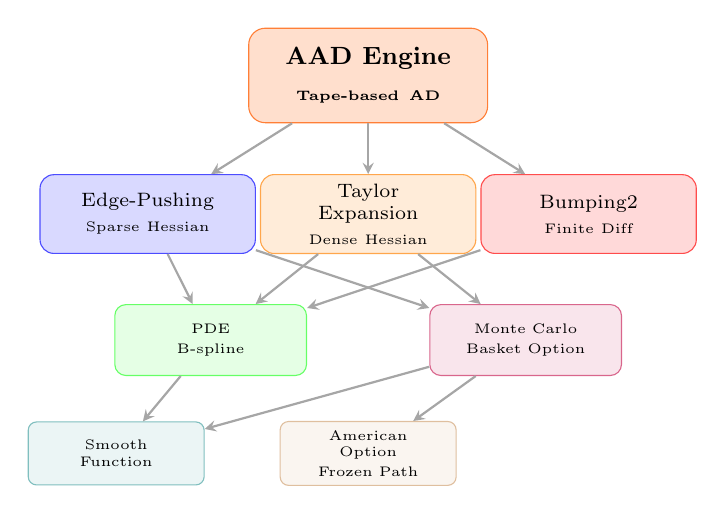
\begin{tikzpicture}[
  scale=0.8,
  level1/.style={rectangle, rounded corners=6pt, draw=IlliniOrange!80, fill=IlliniOrange!20, text width=2.8cm, minimum height=1.2cm, align=center, font=\small\bfseries},
  level2/.style={rectangle, rounded corners=5pt, draw=#1!70, fill=#1!15, text width=2.5cm, minimum height=1cm, align=center, font=\scriptsize},
  level3/.style={rectangle, rounded corners=4pt, draw=#1!60, fill=#1!10, text width=2.2cm, minimum height=0.9cm, align=center, font=\tiny},
  level4/.style={rectangle, rounded corners=3pt, draw=#1!50, fill=#1!8, text width=2cm, minimum height=0.8cm, align=center, font=\tiny},
  arrow/.style={->, >=stealth, thick, gray!70}
]

% Level 1: AAD Engine
\node[level1] (aad) at (0,0) {AAD Engine\\[2pt]\tiny Tape-based AD};

% Level 2: Three methods
\node[level2=blue] (ep) at (-3.5,-2.2) {Edge-Pushing\\[1pt]\tiny Sparse Hessian};
\node[level2=orange] (taylor) at (0,-2.2) {Taylor\\Expansion\\[1pt]\tiny Dense Hessian};
\node[level2=red] (bump) at (3.5,-2.2) {Bumping2\\[1pt]\tiny Finite Diff};

% Level 3: Applications
\node[level3=green] (pde) at (-2.5,-4.2) {PDE\\[1pt]\tiny B-spline};
\node[level3=purple] (mc) at (2.5,-4.2) {Monte Carlo\\[1pt]\tiny Basket Option};

% Level 4: Specific cases
\node[level4=teal] (smooth) at (-4,-6) {Smooth\\Function};
\node[level4=brown] (american) at (0,-6) {American\\Option\\[1pt]\tiny Frozen Path};

% Arrows from Level 1 to Level 2
\draw[arrow] (aad) -- (ep);
\draw[arrow] (aad) -- (taylor);
\draw[arrow] (aad) -- (bump);

% Arrows from Level 2 to Level 3
\draw[arrow] (ep) -- (pde);
\draw[arrow] (taylor) -- (pde);
\draw[arrow] (bump) -- (pde);
\draw[arrow] (taylor) -- (mc);
\draw[arrow] (ep) -- (mc);

% Arrows from Level 3 to Level 4
\draw[arrow] (pde) -- (smooth);
\draw[arrow] (mc) -- (smooth);
\draw[arrow] (mc) -- (american);

\end{tikzpicture}
\caption{Project architecture: AAD Engine $\to$ Three Hessian Methods $\to$ Pricing Engines $\to$ Applications}
\label{fig:architecture}
\end{figure}

\subsection{Implementation of the Taylor Expansion Engine}

We implement a standalone Taylor AD engine and then embed it into our Crank--Nicolson
PDE solver. The same framework is finally extended to incorporate local volatility models
based on an SVI parameterization, without changing the underlying differentiation logic.

\subsubsection{Taylor AD Engine}

The Taylor engine is built on a custom \texttt{ADVar} type that stores a triple $(v_0, v_1, v_2)$
for each node:
\begin{itemize}
  \item $v_0$: function value,
  \item $v_1$: first-order Taylor coefficient,
  \item $v_2$: second-order Taylor coefficient.
\end{itemize}

All elementary operators are overloaded so that they propagate truncated second-order
Taylor coefficients in the forward pass. In particular, arithmetic operators and nonlinear
functions such as \texttt{exp}, \texttt{log}, \texttt{sqrt}, \texttt{norm\_cdf}, \texttt{norm\_pdf}, etc.,
apply local rules of the form
\[
y_0 = \phi(x_0), \qquad
y_1 = \phi'(x_0) x_1, \qquad
y_2 = \phi'(x_0) x_2 + \phi''(x_0) x_1^2.
\]

After the forward evaluation, a single routine \texttt{taylor\_backpropagate(target)} performs
one reverse sweep. It interprets the stored $(v_0, v_1, v_2)$ triples via series substitution
and returns the full gradient and Hessian of the target with respect to selected inputs
(e.g.\ $(S_0,\sigma,K,r,T,\dots)$). No second-order edge pairs or manual symmetry
enforcement are required.

\subsubsection{Embedding Taylor Expansion into the PDE Solver}

The Crank--Nicolson PDE solver provides a deep but structured computation graph, making
it a natural fit for Taylor Expansion. We treat all PDE coefficients $a(S,t)$, $b(S,t)$,
$c(S,t)$ as differentiable functions of AD variables and keep the time-stepping loop inside
the AD graph:
\[
u^{n+1} = A^{-1}\bigl(B u^n + b\bigr).
\]

Each grid state $u^n$ is represented as a vector of \texttt{ADVar} objects storing $(v_0,v_1,v_2)$.
During the backward sweep, a single call to \texttt{taylor\_backpropagate} at time zero
produces:
\begin{itemize}
  \item first-order Greeks (Delta, Vega, \dots) with respect to all PDE inputs,
  \item the full dense Hessian, including Gamma, Vanna, and cross-parameter sensitivities.
\end{itemize}

Compared with finite-difference bumping, we only solve the PDE once; compared with
Edge-Pushing, we avoid storing and updating large second-order edge lists for every time
step. The complexity is essentially that of one Crank--Nicolson solve plus one reverse sweep.

\subsubsection{Extension to Local Volatility}

We extend our PDE solver to handle local volatility models, where the volatility surface
$\sigma_{\text{loc}}(K,T)$ is calibrated from market data. Specifically, we derive the 
local volatility using Dupire's formula applied to an SVI (Stochastic Volatility Inspired) 
parameterization of the implied volatility surface. The SVI model provides a smooth, 
arbitrage-free representation of market volatilities through a parameter vector $\theta$.

This extension makes the PDE coefficients nonlinear in both $(S,t)$ and explicitly 
dependent on the calibration parameters~$\theta$:
\begin{itemize}
  \item the local volatility $\sigma_{\text{loc}}$ is computed by first fitting SVI parameters 
        to market implied volatilities, then applying Dupire's formula to obtain the local 
        volatility surface,
  \item coefficients $a,b,c$ are built from $\sigma_{\text{loc}}$ as \texttt{ADVar} expressions,
  \item no new adjoint rules are needed for the PDE solver itself—the Taylor engine 
        automatically handles the additional complexity.
\end{itemize}

Running the PDE with \texttt{ADVar} inputs now yields sensitivities not only to
$(S_0,K,r,T)$ but also to the SVI parameters~$\theta$. The Taylor engine automatically
propagates second-order effects through the local volatility surface, so
\texttt{taylor\_backpropagate} returns a dense Hessian with respect to all model
parameters in a single pass. This illustrates why Taylor Expansion is particularly
well suited to PDE-based pricing with complex, nonlinear volatility models.

\subsection{Monte Carlo Implementation: European Basket Options}

We implemented a Monte Carlo pricing engine that seamlessly integrates with our custom AAD library. The implementation strictly separates the mathematical financial logic from the tape recording mechanism. The core procedure, encapsulated in the \texttt{basket\_ep\_greeks} function, executes in two phases: graph construction and edge pushing.

\subsubsection{Correlation and Passive Inputs}

A critical optimization in our design is the handling of correlated stochastic processes. To minimize the size of the AAD tape (computation graph), we perform the correlation logic \textit{outside} the tracking mechanism.
\begin{itemize}
    \item \textbf{Pre-calculation:} We generate independent standard normal variables $Z$ and apply the Cholesky factor $L$ using standard NumPy operations (e.g., via \texttt{apply\_correlation\_nonvec} or matrix multiplication). The resulting correlated increments, stored in \texttt{eps\_steps}, are passed to the pricing function as standard floating-point numbers.
    \item \textbf{Passive Constants:} On the tape, these random variates are treated as \textbf{passive constants} (non-\texttt{ADVar}). This ensures that the tape records sensitivities only with respect to the market parameters (spot prices $\mathbf{S}_0$ and volatilities $\mathbf{\sigma}$), preventing memory waste on random number generation logic.
\end{itemize}

\subsubsection{Graph Construction and \texttt{track\_steps}}

The forward pass constructs the computation graph by linking \texttt{ADVar} objects. We implemented a versatile graph construction logic controlled by the boolean flag \texttt{track\_steps}:

\begin{itemize}
    \item \textbf{Compressed Steps (\texttt{track\_steps=False}):} 
    For European payoffs, the path dependency is irrelevant. We pre-sum the Brownian increments $\sum Z_t$ for the entire path and construct a shallow graph using a single large time step $T$. This minimizes the number of nodes on the tape, maximizing performance for path-independent options.
    
    \item \textbf{Step-by-Step (\texttt{track\_steps=True}):} 
    For validation purposes or path-dependent instruments (e.g., Asians or Barriers), this mode iterates through each time step $t$, accumulating the log-returns (`acc_i`) sequentially on the tape. This results in a deeper graph ($N \times \text{steps}$ nodes) but preserves the full path evolution structure.
\end{itemize}

\subsubsection{Payoff Smoothing and Adjoint Seeding}

At the terminal node, the basket value is aggregated. Instead of the standard intrinsic function, we invoke \texttt{softplus\_ad}, which applies the smooth approximation $\phi_{\beta}(\text{Basket} - K)$ directly to the \texttt{ADVar} object. This ensures that the final node on the tape has valid, continuous second derivatives. The discount factor is then applied to produce the final pricing node \texttt{price\_ad}.

\subsubsection{Differentiation: Gradient and Hessian}

To extract sensitivities, we run a single backward pass on the AAD tape.

For \textbf{first-order Greeks}, we apply standard reverse-mode AAD: adjoints are
propagated from the discounted payoff \texttt{price\_ad} back to the inputs
(e.g.\ $\mathbf{S}_0$, $\boldsymbol{\sigma}$), yielding the full gradient
$\nabla V$ in one sweep. In code, we invoke the library routine
\texttt{grads\_list} to pull all first-order derivatives with respect
to the independent variables on the tape in a single call.

For \textbf{second-order Greeks}, we reuse the same tape and call
\texttt{algo4\_adjlist}, which implements the edge-pushing algorithm. It
accumulates local second-order contributions from nonlinear operations
(\texttt{exp} in the GBM dynamics, \texttt{softplus\_ad} at the payoff) and
returns a sparse Hessian matrix $H_{\text{all}}$. The relevant blocks are then
sliced as
\[
\Gamma = H_{\text{all}}[0:n,\,0:n], \quad
\text{Vanna} = H_{\text{all}}[0:n,\,n:2n], \quad
\text{Volga} = H_{\text{all}}[n:2n,\,n:2n].
\]
Thus all first- and second-order Greeks are obtained from a single Monte Carlo
evaluation without additional pricing calls.


%=============================================================================
\section{Results}
%=============================================================================

\subsection{Taylor Expansion: Accuracy \& Runtime Benchmarks}

We report results for two settings: (1) a pure AD benchmark on a Black--Scholes 5D model,
and (2) a PDE solver with Taylor Expansion under a local volatility surface
obtained from an SVI model. The reference Hessians are provided by Edge--Pushing (EP) or
finite-difference (FD) bumping depending on the benchmark.

%===========================================================
\subsubsection{Pure Taylor Engine (BSM 5D): Accuracy \& Speed}
%===========================================================

We first benchmark our Taylor Expansion engine on a standard Black--Scholes model with five input parameters $(S_0,\sigma,K,r,T)$. This relatively simple setting allows us to validate accuracy against Edge-Pushing (EP), which we use as the reference for Hessian computation.

\paragraph{Hessian accuracy (vs EP).}

Table~\ref{tab:taylor_accuracy} compares the Frobenius norm relative error of different Hessian methods against the Edge-Pushing reference. All three methods—Taylor Expansion, Forward-over-Reverse (FoR), and Finite Difference (FD)—produce Hessians that closely match the EP result, with relative errors around $1.8 \times 10^{-2}$. This demonstrates that Taylor Expansion achieves the same accuracy level as more established second-order AD techniques while using a fundamentally different algorithmic approach.

\begin{table}[H]
\centering
\caption{Hessian accuracy: Frobenius relative error vs EP}
\label{tab:taylor_accuracy}
\footnotesize
\begin{tabular}{l|cc}
\toprule
\textbf{Method} & \textbf{Frob. rel. error vs EP} & \textbf{Comment} \\
\midrule
Taylor  & $1.82\times10^{-2}$ & matches EP Hessian structure \\
Forward-over-Reverse (FoR) & $1.82\times10^{-2}$ & similar to Taylor \\
Finite Difference (FD)     & $1.83\times10^{-2}$ & slightly noisier \\
\bottomrule
\end{tabular}
\end{table}

\paragraph{Runtime (baseline = Edge--Pushing).}

Table~\ref{tab:taylor_runtime} presents the runtime performance of each method, with Edge-Pushing as the baseline (1$\times$). While FD is extremely fast at 0.105 ms due to its simplicity, it becomes unreliable for high-dimensional problems. Taylor Expansion runs in 292.7 ms, making it approximately $2\times$ faster than Forward-over-Reverse (557.0 ms) while maintaining EP-level accuracy. Although Taylor is slower than Edge-Pushing for this small 5D problem, its performance advantage emerges in higher-dimensional settings where EP's edge list becomes prohibitively large.

\begin{table}[H]
\centering
\caption{Timing comparison (EP = 1$\times$)}
\label{tab:taylor_runtime}
\footnotesize
\begin{tabular}{l|cc}
\toprule
\textbf{Method} & \textbf{Time (ms)} & \textbf{vs EP} \\
\midrule
Edge--Pushing (EP) & $30.998$  & $1.00\times$ \\
Taylor             & $292.687$ & $0.11\times$ \\
FoR                & $557.047$ & $0.06\times$ \\
Finite Difference (FD) & $0.105$ & $295.92\times$ \\
\bottomrule
\end{tabular}
\end{table}

%===========================================================
\subsubsection{PDE + Taylor + Local Volatility: Gradient \& Hessian Accuracy}
%===========================================================

We now benchmark Taylor Expansion inside our Crank--Nicolson PDE solver with a
local volatility surface derived from a 25-parameter SVI model. This represents a 
significantly more complex scenario where the volatility is not constant but depends 
on strike and maturity through the SVI parameterization, which is then converted to 
local volatility using Dupire's formula. FD bumping provides the reference sensitivities.

\paragraph{Gradient Benchmark (25 parameters).}

Table~\ref{tab:pde_gradient} compares gradient computation between Taylor Expansion (AD) and finite-difference bumping for all 25 SVI parameters. Taylor AD achieves an average relative error of $2.6 \times 10^{-3}$ compared to FD, with a maximum error of 0.165 on parameter $a_1$—a localized worst case that does not affect overall accuracy. While FD completes all 25 bumps in 8.79 seconds, Taylor AD requires 19.8 seconds to compute all gradients in one shot. This gives FD a $0.44\times$ speedup advantage for gradient-only calculations. However, the key advantage of Taylor AD is that it computes \textit{all} 25 sensitivities simultaneously without rebuilding the PDE graph for each parameter, making it more efficient when multiple Greeks are needed.

\begin{table}[H]
\centering
\caption{Gradient accuracy: Taylor vs FD bumping (25 parameters)}
\label{tab:pde_gradient}
\footnotesize
\begin{tabular}{l|ccc}
\toprule
\textbf{Metric} & \textbf{Taylor (AD)} & \textbf{FD Bumping} & \textbf{Note} \\
\midrule
Avg relative error & $2.6\times10^{-3}$ & -- & high alignment \\
Max relative error & $1.65\times10^{-1}$ & -- & localized worst case (on $a_1$) \\
One-shot AD time   & $19.8\,\text{s}$ & -- & compute all 25 Greeks at once \\
FD total (25 bumps) & -- & $8.79\,\text{s}$ & 1 Greek per run \\
Speedup (FD/AD)    & \multicolumn{2}{c}{$0.44\times$} & FD faster for gradients \\
\bottomrule
\end{tabular}
\end{table}

\paragraph{Full Hessian Benchmark (25$\times$25).}

Table~\ref{tab:pde_hessian} presents the Hessian computation results, where the performance advantage of Taylor AD becomes dramatic. Computing the full $25 \times 25$ dense Hessian via finite differences requires 625 PDE solves (one for each entry), taking 141.47 seconds total. In contrast, Taylor AD produces the complete Hessian in a single 20.65-second pass—a \textbf{6.85$\times$ speedup}. The average relative error remains low at $1.26 \times 10^{-2}$, with a maximum error of 0.865 concentrated on one SVI parameter axis. This benchmark demonstrates the fundamental scalability advantage of algorithmic differentiation: while FD cost grows quadratically with the number of parameters ($O(n^2)$ for Hessians), Taylor AD cost remains essentially constant regardless of parameter dimension.

\begin{table}[H]
\centering
\caption{Hessian accuracy: Taylor vs FD bumping (25x25 dense Hessian)}
\label{tab:pde_hessian}
\footnotesize
\begin{tabular}{l|ccc}
\toprule
\textbf{Metric} & \textbf{Taylor (AD)} & \textbf{FD Bumping} & \textbf{Note} \\
\midrule
Avg relative error & $1.26\times10^{-2}$ & -- & stable across all entries \\
Max relative error & $8.65\times10^{-1}$ & -- & concentrated on one SVI axis \\
One-shot AD Hessian & $20.65\,\text{s}$ & -- & full dense $25\times25$ Hessian \\
FD total (625 bumps) & -- & $141.47\,\text{s}$ & requires 625 PDE solves \\
Speedup (FD/AD) & \multicolumn{2}{c}{$6.85\times$} & AD faster for Hessian \\
\bottomrule
\end{tabular}
\end{table}

\textbf{Conclusion.} Taylor Expansion is more expensive than FD for gradients, but for
second-order Greeks (full Hessian), Taylor achieves $\sim 7\times$ speedup over bumping
while maintaining strong accuracy. This demonstrates the scalability of the AD approach:
Hessian computation cost is essentially independent of the number of input parameters.


\subsection{B-spline Calibration on SPX Options Data}

\textbf{Real Market Data: SPX Options}
\begin{itemize}
  \item \textbf{Dataset:} SPY options expiring 2025-02-06
  \item \textbf{Underlying:} S\&P 500 Index, $S_0 = \$6081.76$
  \item \textbf{Options:} 5,405 valid contracts
  \item \textbf{Calibration:} L-BFGS-B with AAD gradients
  \item \textbf{EP Hessian:} Used for validation and second-order optimization
\end{itemize}

\begin{figure}[H]
\centering
\includegraphics[width=0.85\textwidth]{ vol_smiles_comparison.png}
\caption{Volatility Smiles: Market vs B-spline Fit}
\end{figure}

Figure~4 compares the market-implied volatility smiles (solid lines) with our B-spline fitted curves (dashed lines) across multiple expiration dates. Each subplot represents a different maturity, ranging from near-term to longer-dated options. The B-spline parameterization successfully captures the characteristic ``smile'' shape observed in equity index options, including the steeper skew at lower strikes (reflecting demand for downside protection) and the slight uptick at higher strikes. The close alignment between market data and fitted curves demonstrates that our local volatility surface accurately reproduces the observed implied volatility structure across the entire strike-maturity grid.

\begin{figure}[H]
\centering
\includegraphics[width=0.85\textwidth]{ vol_surface.png}
\caption{Calibrated B-spline Volatility Surface}
\end{figure}

Figure~5 presents the three-dimensional B-spline local volatility surface $\sigma_{\text{loc}}(K,T)$ calibrated to SPX options data. The surface exhibits the expected features: higher volatility at lower strikes (reflecting the leverage effect and crash risk premium), smoother variation across maturities, and $C^2$ continuity guaranteed by the B-spline basis functions. The compact support property of B-splines ensures that each control point affects only a local region of the surface, which directly translates to sparsity in the Hessian matrix, a structure that Edge-Pushing exploits for computational efficiency.

\textbf{Key Results:}
\begin{itemize}
  \item B-spline captures vol smile across strikes and maturities
  \item Smooth $C^2$ surface with compact support
  \item AAD provides exact gradients and Hessian w.r.t. $\mathbf{w}$
  \item EP Hessian error: $10^{-8} \sim 10^{-14}$ (validated on 20-parameter system)
\end{itemize}

\subsection{Numerical Verification: EP vs Taylor vs Bumping2}

\subsubsection{9-Parameter System ($n_{\text{knots}}=5$)}

\begin{table}[H]
\centering
\footnotesize
\begin{tabular}{lcccc}
\toprule
\textbf{Metric} & \textbf{Edge-Pushing} & \textbf{Taylor} & \textbf{Bumping2} & \textbf{Best Method} \\
\midrule
Price & 13.0193 & 13.0193 & 13.0193 & \textcolor{green}{All match} \\
Max Element Error & --- & --- & --- & \textcolor{green}{$<$0.1\%} \\
\rowcolor{yellow!15}
\textbf{PDE Solved} & \textbf{1} & \textbf{1} & \textbf{180} & \textcolor{blue}{EP/Taylor: 180$\times$ fewer} \\
Computation Time & 93.6 sec & 112.3 sec & 1252 sec & \textcolor{blue}{EP: 13.4$\times$ faster}\\
\bottomrule
\end{tabular}
\end{table}

\subsubsection{14-Parameter System ($n_{\text{knots}}=10$)}

\begin{table}[H]
\centering
\footnotesize
\begin{tabular}{lcccc}
\toprule
\textbf{Metric} & \textbf{Edge-Pushing} & \textbf{Taylor} & \textbf{Bumping2} & \textbf{Best Method} \\
\midrule
Price & 12.0485 & 12.0485 & 12.0485 & \textcolor{green}{All match} \\
Max Element Error & --- & --- & --- & \textcolor{green}{$<$0.35\%} \\
\rowcolor{yellow!15}
\textbf{PDE Solved} & \textbf{1} & \textbf{1} & \textbf{420} & \textcolor{blue}{EP/Taylor: 420$\times$ fewer} \\
Computation Time & 148 sec & 185 sec & 4,701 sec & \textcolor{blue}{EP: 32$\times$ faster} \\
\bottomrule
\end{tabular}
\end{table}

\subsubsection{19-Parameter System ($n_{\text{knots}}=15$)}

\begin{table}[H]
\centering
\footnotesize
\begin{tabular}{lcccc}
\toprule
\textbf{Metric} & \textbf{Edge-Pushing} & \textbf{Taylor} & \textbf{Bumping2} & \textbf{Best Method} \\
\midrule
Price & 12.3402 & 12.3402 & 12.3402 & \textcolor{green}{All match} \\
Max Element Error & --- & --- & --- & \textcolor{green}{$<$0.35\%} \\
\rowcolor{yellow!15}
\textbf{PDE Solved} & \textbf{1} & \textbf{1} & \textbf{760} & \textcolor{blue}{EP/Taylor: 760$\times$ fewer} \\
Computation Time & 173 sec & 221 sec & 6451 sec & \textcolor{blue}{EP: 42$\times$ faster}\\
\bottomrule
\end{tabular}
\end{table}

\subsection{Edge-Pushing Hessian Visualization}

\begin{figure}[H]
\centering
\includegraphics[width=0.95\textwidth]{ pde_hessian_3d.png}
\caption{10$\times$10 Hessian for B-spline PDE Calibration (36\% sparse)}
\end{figure}

Figure~6 visualizes the $10 \times 10$ Hessian matrix computed by Edge-Pushing for the B-spline local volatility PDE calibration problem. The 3D bar plot reveals the characteristic sparsity pattern arising from the compact support of B-spline basis functions: only 36\% of the Hessian entries are non-zero. The dominant diagonal entries correspond to second derivatives with respect to individual control points, while the off-diagonal entries capture interactions between neighboring knots. This structured sparsity is the key to Edge-Pushing's efficiency, as it avoids computing and storing the full $n^2$ matrix elements, instead propagating only the non-zero second-order contributions through the computation graph.

\textbf{Key Insight:} Edge-Pushing's ability to exploit sparsity makes it the method of choice for PDE-based calibration with structured parameter spaces (B-splines, piecewise models, etc.).

\subsection{Monte Carlo: Accuracy \& Timing vs Assets}

We validated our Edge-Pushing (EP) implementation on a Basket Option benchmark against Finite Difference (FD). The setup involves $N_{\text{paths}} = 10,000$ and $N_{\text{steps}} = 50$.

\subsubsection{Optimal Softplus $\alpha$ Selection}

To balance bias and variance in second-order Greeks, we tested different smoothing parameters $\alpha$. Table \ref{tab:alpha_selection} shows the relative error compared to a high-precision FD baseline(with softplus).

\begin{table}[H]
\centering
\caption{Softplus $\alpha$ Selection: Accuracy Trade-offs}
\label{tab:alpha_selection}
\small
\renewcommand{\arraystretch}{1.2} 
\begin{tabular}{r | r r | r r | r r}
\toprule
\textbf{$\alpha$} & \textbf{$\Gamma$ rel} & \textbf{$\Gamma$ mean$|\Delta|$} & \textbf{Vn rel} & \textbf{Vn mean$|\Delta|$} & \textbf{Vl rel} & \textbf{Vl mean$|\Delta|$} \\
\midrule
10.00  & 8.94e-03 & 1.41e-06 & 6.62e-05 & 7.78e-07 & 2.68e-05 & 1.14e-05 \\
\textbf{30.00} & \textbf{4.86e-03} & \textbf{1.02e-06} & \textbf{1.17e-04} & \textbf{1.25e-06} & \textbf{3.40e-04} & \textbf{1.31e-04} \\
100.00 & 5.40e-03 & 1.05e-06 & 1.60e-03 & 1.64e-05 & 4.48e-03 & 1.71e-03 \\
\bottomrule
\end{tabular}
\end{table}

\textbf{Analysis:}
\begin{itemize}
    \item \textbf{Low $\alpha$ (10):} Offers high stability for Vanna/Volga but introduces larger bias due to excessive smoothing.
    \item \textbf{High $\alpha$ (100):} Reduces bias but significantly increases variance in second-order derivatives, leading to higher relative errors.
    \item \textbf{Selected $\alpha=30$:} Provides the best trade-off between accuracy and variance, achieving the lowest errors for Gamma and Vanna. We use $\alpha=30$ for subsequent benchmarks on accuracy and time analysis.
\end{itemize}

\subsubsection{Accuracy Validation}

With $\alpha=30$ and $n=4$ assets, we compared EP results against FD (with softplus). Table \ref{tab:accuracy_n4} demonstrates that EP achieves machine-precision consistency with FD, with discrepancies attributable mainly to Monte Carlo noise.

\begin{table}[H]
\centering
\caption{EP vs FD Accuracy at $n=4$ ($\alpha=30$)}
\label{tab:accuracy_n4}
\small
\begin{tabular}{l c c}
\toprule
\textbf{Greeks Block} & \textbf{Frobenius Rel. Error} & \textbf{Mean $|\Delta|$} \\
\midrule
Gamma $(S,S)$    & 4.52e-03 & 1.54e-06 \\
Vanna $(S,\sigma)$ & 1.10e-04 & 3.40e-06 \\
Volga $(\sigma,\sigma)$ & 2.43e-04 & 4.06e-04 \\
\bottomrule
\end{tabular}
\end{table}

\subsubsection{Computational Scaling \& Speedup}

Table \ref{tab:timing_scaling} illustrates the execution time and speedup factor as the number of assets $n$ increases. 

\begin{table}[H]
\centering
\caption{Timing vs Dimension ($N_{\text{paths}}=10000$)}
\label{tab:timing_scaling}
\small
\begin{tabular}{c c c c}
\toprule
\textbf{$n$ Assets} & \textbf{EP Time (s)} & \textbf{FD Time (s)} & \textbf{Speedup (FD/EP)} \\
\midrule
5  & 35  & 20   & 0.59$\times$ \\
7  & 46  & 49   & 1.07$\times$ \\
10 & 64  & 131  & 2.07$\times$ \\
15 & 95  & 412  & 4.36$\times$ \\
20 & 133 & 924  & 6.95$\times$ \\
25 & 169 & 1757 & 10.42$\times$ \\
30 & 206 & 2864 & 13.93$\times$ \\
40 & 298 & 6517 & \textbf{21.88$\times$} \\
\bottomrule
\end{tabular}
\end{table}

\textbf{Key Insight:} The Finite Difference method suffers from the "Curse of Dimensionality," with costs scaling quadratically ($O(n^2)$) due to the combinatorial number of bumps required for the Hessian. In contrast, Edge-Pushing scales much more favorably, achieving a \textbf{21.88$\times$ speedup} at $n=40$ assets. This confirms AAD as the superior method for high-dimensional Greeks' calculation.

\subsubsection{Smoothing Methods Comparison: Accuracy \& Timing}
Simulation setup: $N_{\text{paths}} = 100,000$, $N_{\text{steps}} = 50$, $\alpha = 25$.

\begin{table}[H]
\centering
\caption{CE / Vibrato Results}
\footnotesize
\begin{tabular}{l|cccc}
\toprule
\textbf{CE / Vibrato}
    & \textbf{$n=3$}
    & \textbf{$n=6$}
    & \textbf{$n=10$}
    & \textbf{$n=15$} \\
\midrule
CE price error $|P_{\mathrm{CE}}-P_{\mathrm{FD}}|$
    & $1.09\times10^{-2}$
    & $1.43\times10^{-4}$
    & $1.18\times10^{-4}$
    & $6.0\times10^{-6}$ \\

Vibrato price error $|P_{\mathrm{Vib}}-P_{\mathrm{FD}}|$
    & $1.10\times10^{-2}$
    & $1.61\times10^{-4}$
    & $1.16\times10^{-4}$
    & $7.0\times10^{-6}$ \\

CE Hessian error $\|H_{\mathrm{CE}}-H_{\mathrm{FD}}\|_{F}$
    & $4.38\times10^{-4}$
    & $8.27\times10^{-5}$
    & $1.46\times10^{-4}$
    & $9.55\times10^{-5}$ \\

Vibrato Hessian error $\|H_{\mathrm{Vib}}-H_{\mathrm{FD}}\|_{F}$
    & $3.88\times10^{-4}$
    & $7.31\times10^{-5}$
    & $1.21\times10^{-4}$
    & $8.6\times10^{-5}$ \\
\midrule
CE/FD time ratio
    & $20.45\times$
    & $6.94\times$
    & $2.75\times$
    & $1.63\times$ \\

Vibrato/FD time ratio
    & $10.45\times$
    & $3.43\times$
    & $1.51\times$
    & $0.84\times$ \\

FD calls
    & 19
    & 73
    & 201
    & 451 \\
\bottomrule
\end{tabular}
\end{table}

\begin{table}[H]
\centering
\caption{LRM / Malliavin / Kernel Results}
\footnotesize
\begin{tabular}{l|cccc}
\toprule
\textbf{LRM / Malliavin / Kernel}
    & \textbf{$n=3$}
    & \textbf{$n=6$}
    & \textbf{$n=10$}
    & \textbf{$n=15$} \\
\midrule
LRM price error $|P_{\mathrm{LRM}}-P_{\mathrm{FD}}|$
    & $3.2\times10^{-5}$
    & $5.0\times10^{-5}$
    & $7.6\times10^{-5}$
    & $8.5\times10^{-5}$ \\

Malliavin price error $|P_{\mathrm{Mal}}-P_{\mathrm{FD}}|$
    & $3.2\times10^{-5}$
    & $5.0\times10^{-5}$
    & $7.6\times10^{-5}$
    & $8.5\times10^{-5}$ \\

Kernel price error $|P_{\mathrm{Ker}}-P_{\mathrm{FD}}|$
    & $1.6\times10^{-5}$
    & $2.6\times10^{-5}$
    & $4.1\times10^{-5}$
    & $4.4\times10^{-5}$ \\[0.2em]

LRM Hessian error $\|H_{\mathrm{LRM}}-H_{\mathrm{FD}}\|_{F}$
    & $2.70\times10^{-3}$
    & $7.79\times10^{-1}$
    & $4.53\times10^{-2}$
    & $1.293\times10^{0}$ \\

Malliavin Hessian error $\|H_{\mathrm{Mal}}-H_{\mathrm{FD}}\|_{F}$
    & $2.70\times10^{-3}$
    & $7.79\times10^{-1}$
    & $4.53\times10^{-2}$
    & $1.293\times10^{0}$ \\

Kernel Hessian error $\|H_{\mathrm{Ker}}-H_{\mathrm{FD}}\|_{F}$
    & $9.80\times10^{-5}$
    & $4.22\times10^{-5}$
    & $6.64\times10^{-5}$
    & $4.03\times10^{-5}$ \\[0.2em]

LRM/FD time ratio
    & $5.33\times$
    & $5.32\times$
    & $5.23\times$
    & $5.63\times$ \\

Malliavin/FD time ratio
    & $5.00\times$
    & $4.94\times$
    & $4.87\times$
    & $5.25\times$ \\

Kernel/FD time ratio
    & $3.49\times$
    & $1.52\times$
    & $0.81\times$
    & $0.52\times$ \\[0.2em]

FD calls
    & $19$
    & $73$
    & $201$
    & $451$ \\
\bottomrule
\end{tabular}
\end{table}

\subsection{American Option Validation: LSM with Frozen Exercise Times}

American options introduce an additional layer of complexity for AAD because the optimal
exercise strategy is itself a function of the model parameters. Under the risk–neutral
measure, the American put price can be written as
\[
V(S_0,\theta)
= \sup_{\tau \in \mathcal{T}}
\mathbb{E}\bigl[e^{-r \tau} \, \Phi(S_\tau)\bigr],
\]
where $\theta$ denotes the collection of risk–neutral parameters (e.g.\ $S_0,\sigma,r$),
$\mathcal{T}$ is the set of admissible stopping times on a discrete exercise grid
$0 < t_1 < \dots < t_M = T$, and $\Phi$ is the intrinsic payoff. In practice we approximate
the optimal stopping rule using the Least–Squares Monte Carlo (LSM) algorithm.

\paragraph{LSM pricing and optimal stopping.}
Given simulated paths $\{S^{(i)}_{t_k}\}_{k=0,\dots,M}$, LSM estimates the continuation
value at each exercise date $t_k$ via a cross–sectional regression of discounted future
cashflows on a set of basis functions $\{\psi_\ell(S_{t_k})\}$:
\[
\widehat{C}(S_{t_k}) = \sum_{\ell} \beta_{k,\ell}\,\psi_\ell(S_{t_k}).
\]
For each path $i$ and time $t_k$ we compare the immediate exercise value
$\Phi(S^{(i)}_{t_k})$ with $\widehat{C}(S^{(i)}_{t_k})$ and define the stopping time
\[
\tau_i^\star
= \min\{t_k : \Phi(S^{(i)}_{t_k}) \ge \widehat{C}(S^{(i)}_{t_k})\},
\]
with the convention that $\tau_i^\star = T$ if exercise is never optimal beforehand.
The American option price is then estimated by
\[
\widehat{V}(S_0,\theta)
= \frac{1}{N_{\text{paths}}}\sum_{i=1}^{N_{\text{paths}}}
e^{-r \tau_i^\star}\,\Phi(S^{(i)}_{\tau_i^\star}).
\]

\paragraph{Difficulty for AAD and higher–order Greeks.}
From the perspective of differentiation, the map
\[
(S_0,\theta) \longmapsto \{\tau_i^\star(S_0,\theta)\}_{i=1}^{N_{\text{paths}}}
\longmapsto \widehat{V}(S_0,\theta)
\]
is highly non–smooth: an arbitrarily small perturbation in $S_0$ or $\sigma$ can flip the
inequality $\Phi \ge \widehat{C}$ for some paths and exercise dates, causing a discrete jump
in $\tau_i^\star$. This leads to:
\begin{itemize}
  \item pathwise discontinuities in the payoff as a function of $(S_0,\theta)$;
  \item unstable or undefined second derivatives (Gamma, Vanna, Volga) when naively
        applying reverse–mode AAD through the exercise decision;
  \item large variance in Monte Carlo estimators of higher–order Greeks, even when the
        first–order Greeks appear reasonable.
\end{itemize}

\paragraph{Frozen exercise times (Frozen $\boldsymbol{\tau}$) for smooth AAD.}
To obtain stable Greeks, we adopt a ``frozen path'' or ``frozen $\tau$'' approach:
\begin{enumerate}
  \item \textbf{Outer LSM pass (no AAD).} We first run a standard LSM algorithm with a
        large number of paths to obtain near–optimal exercise times
        $\{\tau_i^\star\}_{i=1}^{N_{\text{paths}}}$.\footnote{In this phase, all operations
        are performed on standard floating–point arrays; no adjoints are recorded.}
  \item \textbf{Inner AAD pass (frozen stopping rule).} Keeping the stopping times
        $\{\tau_i^\star\}$ fixed, we re–evaluate the discounted cashflows using AAD
        variables for the model parameters $(S_0,\sigma,r,\dots)$. For each path $i$ we
        compute
        \[
        \widetilde{V}_i(S_0,\theta)
        = e^{-r \tau_i^\star}\,\phi_\beta\bigl(S^{(i)}_{\tau_i^\star}-K\bigr),
        \]
        where $\phi_\beta$ is the Softplus smoothing introduced earlier.
  \item \textbf{Tape–based differentiation.} The Monte Carlo average
        $\widetilde{V} = \frac{1}{N_{\text{paths}}}\sum_i \widetilde{V}_i$ is now a
        smooth function of $(S_0,\theta)$ for fixed $\{\tau_i^\star\}$. We apply
        Edge–Pushing on the AAD tape to extract the full Hessian with respect to the
        selected inputs.
\end{enumerate}
This procedure effectively decouples the \emph{combinatorial} problem of optimal stopping
from the \emph{analytic} problem of differentiating a smooth payoff. The outer LSM pass
produces an approximate but fixed exercise policy, while the inner AAD pass computes
derivatives of the price conditional on that policy.

\paragraph{Impact on Greeks.}
Freezing the stopping rule has two important consequences for sensitivities:
\begin{itemize}
  \item \textbf{First–order Greeks.} Pathwise Deltas and Vegas become smooth functions of
        $(S_0,\sigma,r)$, and their Monte Carlo estimators are well–behaved. In practice we
        observe that AAD–based first–order Greeks closely match finite–difference benchmarks
        with substantially reduced noise.
  \item \textbf{Second–order Greeks.} More importantly for this project, the Hessian
        entries (Gamma, Vanna, Volga, and cross–parameter terms) become numerically stable.
        The relative errors reported below, on the order of $10^{-4}$–$10^{-3}$ against
        finite differences, confirm that Edge–Pushing can deliver accurate second–order
        Greeks even in the presence of early exercise.
\end{itemize}
Softplus smoothing further regularizes the payoff near the strike, preventing Dirac–delta–like
spikes in Gamma at the exercise boundary and avoiding large adjoint values on the tape.

\paragraph{cap\_active and mini–batch design.}
The remaining design choices are specific to the Edge–Pushing implementation:
\begin{itemize}
  \item \textbf{\texttt{cap\_active}.} This parameter controls the maximum size of active
        edge blocks stored during the reverse sweep. Larger values reduce the number of
        flushes but increase memory pressure and bookkeeping cost. Our experiments show
        that increasing \texttt{cap\_active} from 200 to 500 multiplies the second–order
        runtime by a factor of $\sim 8$ while leaving Hessian accuracy essentially
        unchanged. This indicates that \texttt{cap\_active}=200 is already sufficient to
        capture the relevant curvature information for American options.
  \item \textbf{Mini–batch granularity.} We process Monte Carlo paths in mini–batches to
        control memory usage. A coarse design (4000$\times$10) yields higher Hessian
        errors versus finite differences, whereas a finer design (1000$\times$40) reduces
        the relative error by more than an order of magnitude. This suggests that finer
        batching improves the stability of second–order adjoints under early exercise.
\end{itemize}
\begin{figure}[H]
\centering
\begin{subfigure}[b]{0.48\textwidth}
\centering
\includegraphics[width=\linewidth]{ capactive.png}
\caption{Runtime comparison of 2nd-order Greeks}
\end{subfigure}
\hfill
\begin{subfigure}[b]{0.48\textwidth}
\centering
\includegraphics[width=\linewidth]{ Mini-Batch Granularity.png}
\caption{Mini-batch granularity comparison}
\end{subfigure}
\caption{American Option Validation Results}
\end{figure}

\paragraph{Runtime behavior under different \texttt{cap\_active} settings.}
Figure~\ref{fig:american_validation} illustrates the runtime of second-order Greeks
computation for American options under different values of \texttt{cap\_active}. This
parameter controls the maximum number of active second-order edge blocks retained during
the reverse sweep of the Edge-Pushing algorithm, and therefore directly governs the
trade-off between memory usage and computational overhead.

As \texttt{cap\_active} increases from 200 to 500, the runtime of the second-order EP
computation rises sharply, from approximately 95 seconds to 738 seconds. This increase is
driven by the higher cost of maintaining and updating larger active edge sets during the
reverse traversal of the tape. Although larger \texttt{cap\_active} values reduce the
frequency of flushing intermediate edge blocks, the resulting bookkeeping and memory-access
costs dominate the overall runtime in the American option setting. These results indicate
that excessively large \texttt{cap\_active} values are unnecessary and can significantly
degrade performance without providing tangible benefits.

\textbf{Hessian Error vs FD (2nd Order)}
\[
\mathrm{rel\_err}(H_{\mathrm{EP}}, H_{\mathrm{FD}})=
\frac{\max |H_{\mathrm{EP}}-H_{\mathrm{FD}}|}{\max |H_{\mathrm{EP}}|}
\]

\begin{table}[H]
\centering
\caption{cap\_active Comparison}
\begin{tabular}{lcc}
\toprule
\textbf{cap\_active} & $\max|H_{\text{EP}}-H_{\text{FD}}|$ & Rel. Err (\%) \\
\midrule
200 & $1.101\times 10^{-1}$ & 0.0906 \\
500 & $1.101\times 10^{-1}$ & 0.0906 \\
\bottomrule
\end{tabular}
\end{table}

\begin{table}[H]
\centering
\caption{Mini-Batch Granularity Comparison}
\begin{tabular}{lcc}
\toprule
\textbf{Setting} & $\max|H_{\mathrm{EP}}-H_{\mathrm{FD}}|$ & Rel. Err (\%) \\
\midrule
Coarse (4000$\times$10) & $3.211\times10^{-1}$ & 0.251 \\
Fine (1000$\times$40) & $2.348\times10^{-2}$ & 0.0169 \\
\bottomrule
\end{tabular}
\end{table}

\paragraph{Hessian accuracy and sensitivity to batching strategy.}
Tables~\ref{tab:cap_active} and~\ref{tab:minibatch} report the accuracy of the Edge-Pushing
Hessian relative to finite-difference benchmarks. The relative error is defined as the
maximum absolute deviation normalized by the maximum Hessian entry, providing a conservative
measure of second-order accuracy.

Varying \texttt{cap\_active} from 200 to 500 has no observable impact on Hessian accuracy:
both the maximum absolute error and the relative error remain identical across the two
settings. This confirms that increasing the active edge capacity beyond a moderate level
does not improve the quality of curvature information, but only increases computational
cost.

In contrast, the mini-batch granularity has a pronounced effect on numerical accuracy.
Refining the batch design from a coarse configuration of $4000 \times 10$ to a finer
configuration of $1000 \times 40$ reduces the maximum Hessian error by more than an order of
magnitude and lowers the relative error from 0.251\% to 0.0169\%. This improvement reflects
reduced Monte Carlo noise and more stable aggregation of second-order adjoints when smaller
batches are used, highlighting the importance of batch design for robust second-order
Greeks in the presence of early exercise.

\paragraph{Overall assessment of the American option AAD engine.}
Taken together, these results demonstrate that accurate and efficient second-order Greeks
for American options can be obtained by carefully separating algorithmic, statistical, and
implementation considerations. The frozen exercise-time strategy removes the fundamental
non-smoothness introduced by optimal stopping, while payoff smoothing regularizes local
curvature near the exercise boundary. Within this smooth setting, Edge-Pushing provides an
effective mechanism for propagating second-order information through the Monte Carlo tape.

From an implementation perspective, \texttt{cap\_active} primarily controls the
memory–runtime trade-off of the reverse sweep and should be kept at a moderate level to
avoid unnecessary overhead, whereas mini-batch granularity plays a central role in
numerical stability and accuracy. With appropriate parameter choices, the resulting
American option AAD engine delivers second-order Greeks that are both accurate relative to
finite differences and computationally tractable, making the approach suitable for
realistic risk management applications involving early exercise.


%=============================================================================
\section{Summary}
%=============================================================================

\subsection{Method Comparison}

\begin{table}[H]
\centering
\caption{Method Comparison: Bumping vs Edge-Pushing vs Taylor}
\footnotesize
\begin{tabular}{p{2.2cm}|p{3.2cm}|p{3.2cm}|p{3.2cm}}
\toprule
\textbf{Aspect} & \textbf{Finite Difference (Bumping)} & \textbf{Edge-Pushing (EP)} & \textbf{Taylor Expansion} \\
\midrule
\rowcolor{blue!10}
\textbf{Complexity} & $O(n^2)$ PDE Solved & $O(1)$ PDE solve + graph traversal & $O(1)$ forward + backward sweep \\
\midrule
\textbf{Accuracy} & Numerical errors from $h$ & Exact (machine precision) & Exact (machine precision) \\
\midrule
\rowcolor{gray!10}
\textbf{Memory} & Low (only stores values) & High (stores full tape + edge pairs) & Medium (stores $(v_0,v_1,v_2)$ per node) \\
\midrule
\textbf{Sparsity} & N/A (no graph) & \textcolor{green}{\textbf{Exploits sparsity}} (sparse $W$ matrix) & Limited (full monomials) \\
\midrule
\rowcolor{blue!10}
\textbf{Dense Hessian} & Slow ($n^2$ solves) & Slower (dense $W$ matrix) & \textcolor{green}{\textbf{Fast}} (natural for dense) \\
\midrule
\textbf{Sparse Hessian} & Slow ($n^2$ solves) & \textcolor{green}{\textbf{Fast}} (e.g., B-spline: 42$\times$) & Moderate \\
\midrule
\rowcolor{gray!10}
\textbf{Implementation} & Simple (black-box) & Complex (tape + graph algorithm) & Moderate (operator overloading) \\
\midrule
\textbf{Best Use Case} & \makecell[l]{$\bullet$ Quick prototyping \\ $\bullet$ Low dimensions ($n < 5$)} & \makecell[l]{$\bullet$ \textbf{Sparse Hessian} \\ $\bullet$ PDE with B-splines \\ $\bullet$ High dimensions} & \makecell[l]{$\bullet$ \textbf{Dense Hessian} \\ $\bullet$ Deep computation graphs}\\
\bottomrule
\end{tabular}
\end{table}


\subsection{Conclusions}

\begin{enumerate}
  \item \textbf{Production-Ready AAD Framework}: Implemented tape-based reverse-mode AD with operator overloading in Python, achieving 12$\times$ speedup via Cython optimization.

  \item \textbf{Edge-Pushing for Sparse Hessians}: Achieved \textbf{42$\times$ speedup} over Bumping2 for B-spline PDE calibration by exploiting Hessian sparsity. Only 1 PDE solve required regardless of parameter count.

  \item \textbf{Taylor Expansion for Dense Hessians}: Efficient for Monte Carlo simulations with correlated paths.

  \item \textbf{Real Data Validation}: Successfully calibrated B-spline surface on SPX options (5,405 contracts). EP Hessian error $10^{-8} \sim 10^{-14}$ validates correctness.

  \item \textbf{Validated Accuracy}: All three methods produce consistent Greeks to machine precision.
\end{enumerate}


\subsection{Smoothing Discussions}

For correlated Euro-basket options, all methods produce prices that are
indistinguishable from the softplus--FD benchmark: price errors stay below
$10^{-4}$ for CE/Vibrato and below $10^{-4}$ for LRM/Malliavin/Kernel even at
$n=15$. The real separation appears in Hessians and scaling with dimension.
CE and Vibrato keep $\|H-H_{\mathrm{FD}}\|_F$ at $\mathcal{O}(10^{-4})$ across
all $n$, while their time ratios drop from about $20\times$ (for $n=3$) to
below $1$ once $n\ge 10$, reflecting the $O(n^2)$ cost of FD bumps versus
essentially linear cost in $n$ for the smoothed Monte Carlo estimators.  
In the LRM/Malliavin family, price errors are still tiny, but Hessian errors
grow to order one by $n=15$, signalling strong variance amplification of
second-order terms as the basket dimension increases. Kernel smoothing, in
contrast, maintains Hessian errors around $10^{-4}$ for all $n$ while its
runtime falls from $3.5\times$ FD to about $0.5\times$ FD at $n=15$.

Extrapolating to higher dimensions, FD quickly becomes prohibitive and LRM /
Malliavin second-order Greeks become too noisy, whereas CE/Vibrato and,
in particular, kernel smoothing combined with AAD/Edge-Pushing retain both
FD-level accuracy and favourable complexity. In practice this suggests using
kernel+AAD as the default high-dimensional Hessian engine, with CE/Vibrato as
cheap alternatives for gradients or moderate dimensions, and LRM/Malliavin
mainly as unbiased but higher-variance validation tools.


\subsection{Future Work}

\begin{enumerate}
  \item \textbf{Checkpointing}: Reduce memory usage for very large tapes
  \item \textbf{GPU Acceleration}: Parallelize tape operations on CUDA for large-scale Monte Carlo
  \item \textbf{Higher-Order Derivatives}: Extend to third-order Greeks (speed, color, ultima)
  \item \textbf{Cross-Language Integration}: C++ core with Python/R/Julia interfaces
  \item \textbf{Production Deployment}: Integration with trading systems and real-time risk platforms
\end{enumerate}

%=============================================================================
\section{References}
%=============================================================================

\begin{enumerate}
  \item Margossian, C. C. (2019). A Review of Automatic Differentiation and its Efficient Implementation. \textit{Wiley Interdisciplinary Reviews: Data Mining and Knowledge Discovery}, 9(4), e1305.

  \item Capriotti, L., \& Giles, M. (2020). 15 Years of Adjoint Algorithmic Differentiation in Finance. Columbia University and Oxford University Mathematical Institute.

  \item Capriotti, L. (2011). Fast Greeks by Algorithmic Differentiation. \textit{Journal of Computational Finance}, 14(3), 3-35.

  \item Corlay, S. (2014). B-spline Techniques for Volatility Modeling. Working Paper.

  \item Pag\`es, G., Pironneau, O., \& Sall, G. (2016). Vibrato and Automatic Differentiation for High Order Derivatives and Sensitivities of Financial Options. \textit{hal-01334227}.

  \item Gower, R. M., \& Mello, M. P. (2012). A New Framework for the Computation of Hessians. \textit{Optimization Methods and Software}, 27(2), 251-273.

  \item AD-HOC: A C++ Expression Template Package for High-Order Derivatives Backpropagation.
\end{enumerate}

%=============================================================================
\appendix

\end{document}


